\begin{frame}{Materiais e Métodos de Implementação}{Utilização dos Dispositivos em Rede de Comunicações de Dados}

\begin{block}
\small{\justify{Optou-se por utilizar o protocolo de comunicação MQTT com transmissão de dados via Wi-Fi com o uso do protocolo IPV4 e de um servidor local.}}
\end{block}
	
\begin{figure}[htp]
	\centering
	\caption{ \centering{Processo de comunicação através do protocolo MQTT}}
	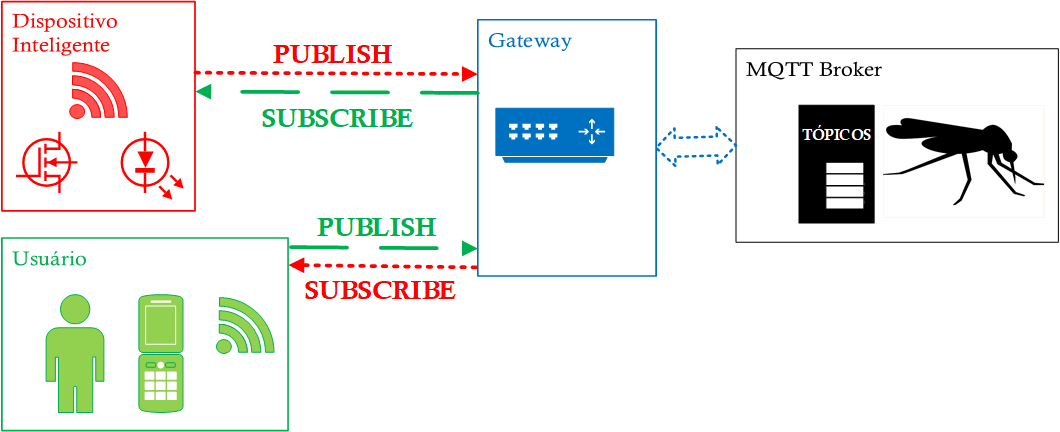
\includegraphics[width=0.9\linewidth]{img/mqtt.png}
    \hspace{1cm}
	\legend{Fonte: Autoria própria}
\end{figure}
\end{frame}

\begin{frame}{Materiais e Métodos de Implementação}{Implementação do \textit{hardware} do ACU-LUM}
\vspace{-0.64cm}
\begin{figure}[htp]
	\centering
	\caption{ \centering\small{{Visão geral da arquitetura de \textit{hardware} do ACU-LUM}}}
	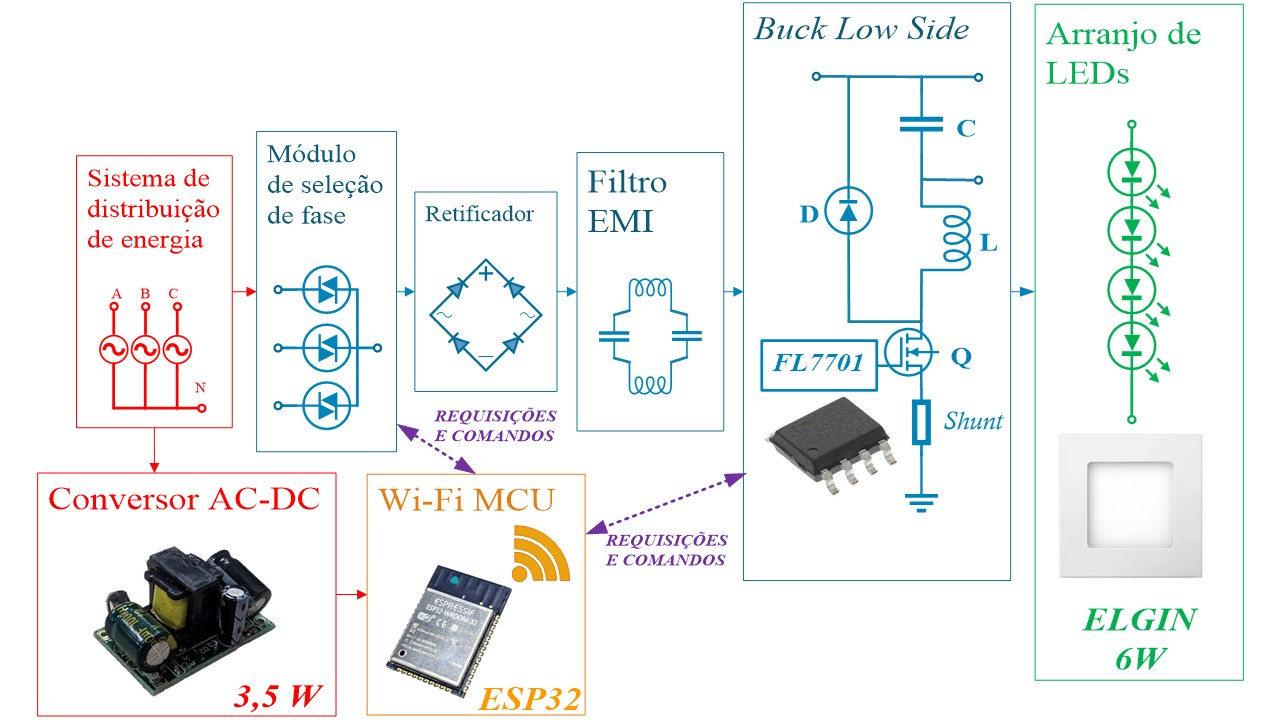
\includegraphics[width=0.98\linewidth]{img/aplum.jpg}
    \hspace{1cm}
    \vspace{3cm}
	\legend{\small{Fonte: Autoria própria}}
\end{figure}
\end{frame}



\begin{frame}{Materiais e Métodos de Implementação}{Implementação do \textit{firmware} do ACU-LUM:  cadastro em rede local}
\vspace{-0.64cm}
\begin{figure}[htp]
	\centering
	\caption{ \centering\small{{Processo de cadastro dos dados de rede no ACU-LUM}}}
	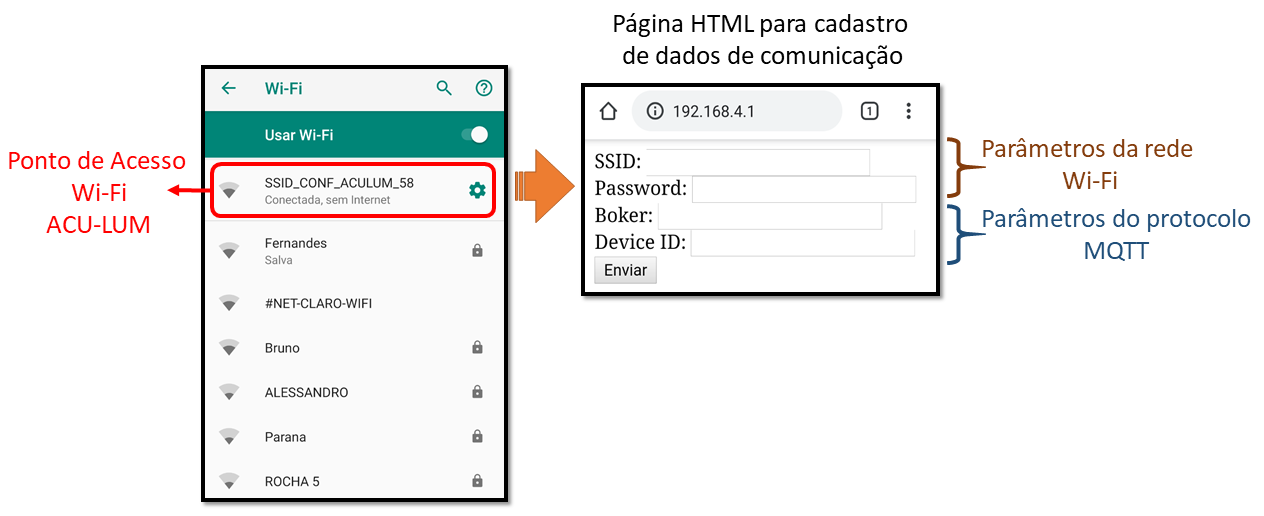
\includegraphics[width=1\linewidth]{img/AP_ESP32.png}
    \hspace{1cm}
    %\vspace{3cm}
	\legend{\small{Fonte: Autoria própria}}
\end{figure}
\end{frame}

\begin{frame}{Materiais e Métodos de Implementação}{Implementação do \textit{firmware} do ACU-LUM: DRFs, ISFs e CSFs}
\vspace{-0.64cm}
\begin{figure}[htp]
	\centering
	\caption{ \centering\small{{Formato JSON de configuração do ACU-LUM}}}
	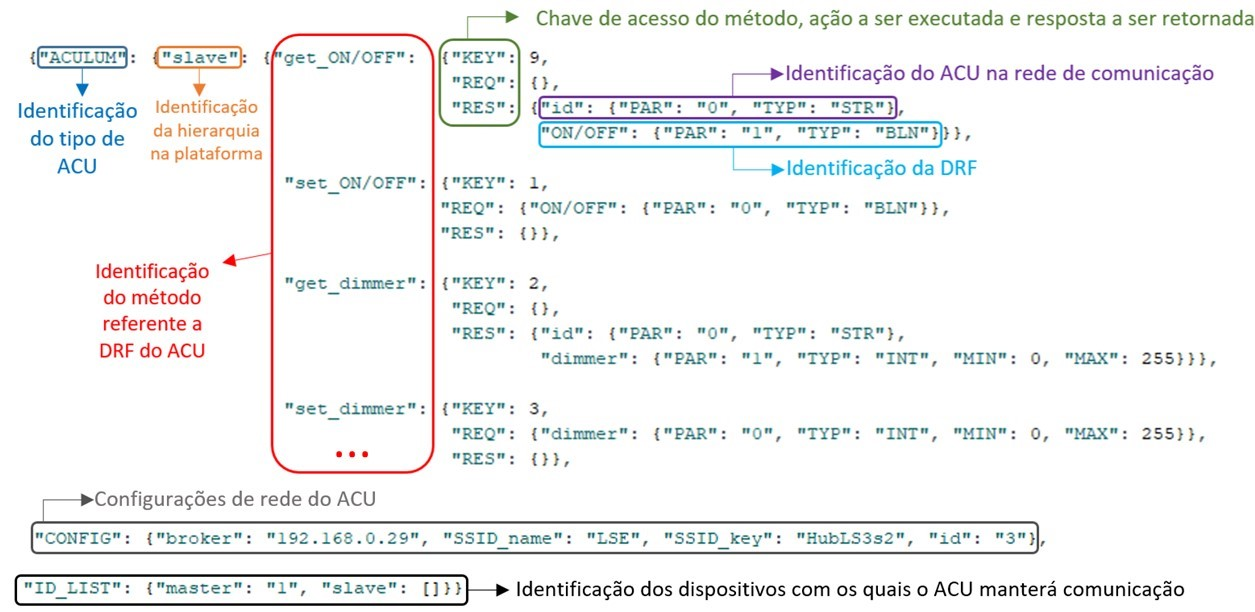
\includegraphics[width=1\linewidth]{img/exjsonLUM.jpg}
    \hspace{1cm}
    %\vspace{1cm}
	\legend{\small{Fonte: Autoria própria}}
\end{figure}
\end{frame}

\begin{frame}{Materiais e Métodos de Implementação}{Implementação do \textit{hardware} do ACU-SB}
%\vspace{-0.64cm}
\begin{figure}[htp]
	\centering
	\caption{ \centering\small{{Visão geral da arquitetura de \textit{hardware} do ACU-SB}}}
	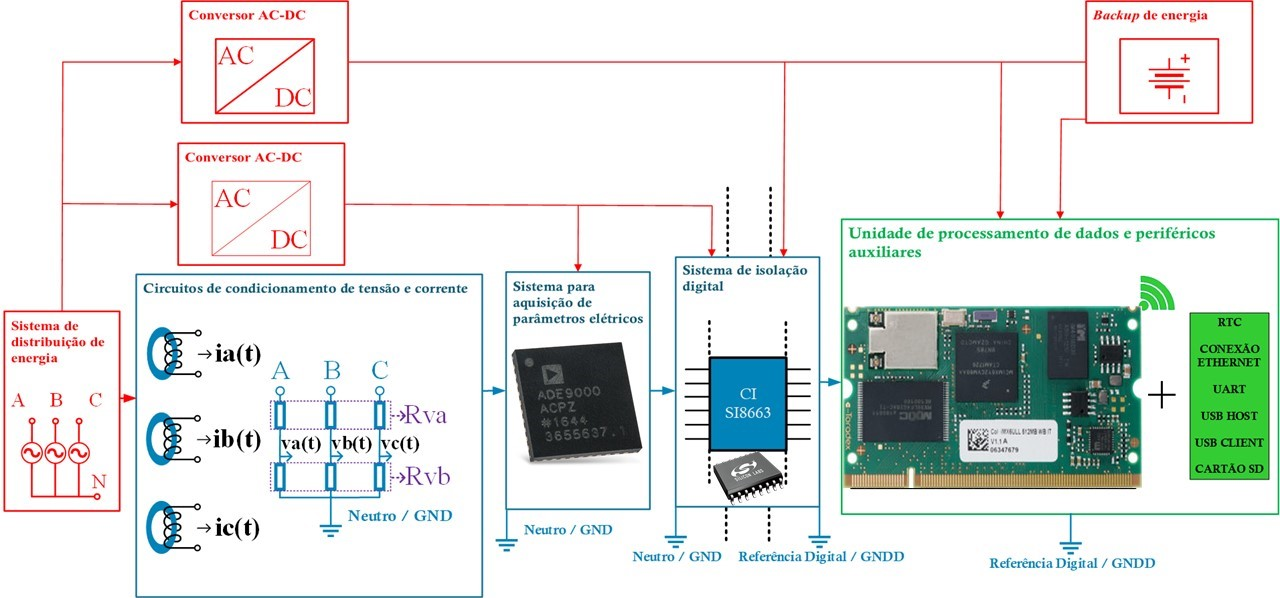
\includegraphics[width=1\linewidth]{img/apSB.jpg}
    \hspace{1cm}
    \vspace{5cm}
	\legend{\small{Fonte: Adaptado \ref{dataISO,ToradexData,ADE9000}}}
\end{figure}
\end{frame}

\begin{frame}{Materiais e Métodos de Implementação}{Implementação do \textit{firmware} do ACU-SB: DRFs, ISFs e CSFs}
\vspace{-0.64cm}
\begin{figure}[htp]
	\centering
	\caption{ \centering\small{{Formato JSON de configuração do ACU-SB}}}
	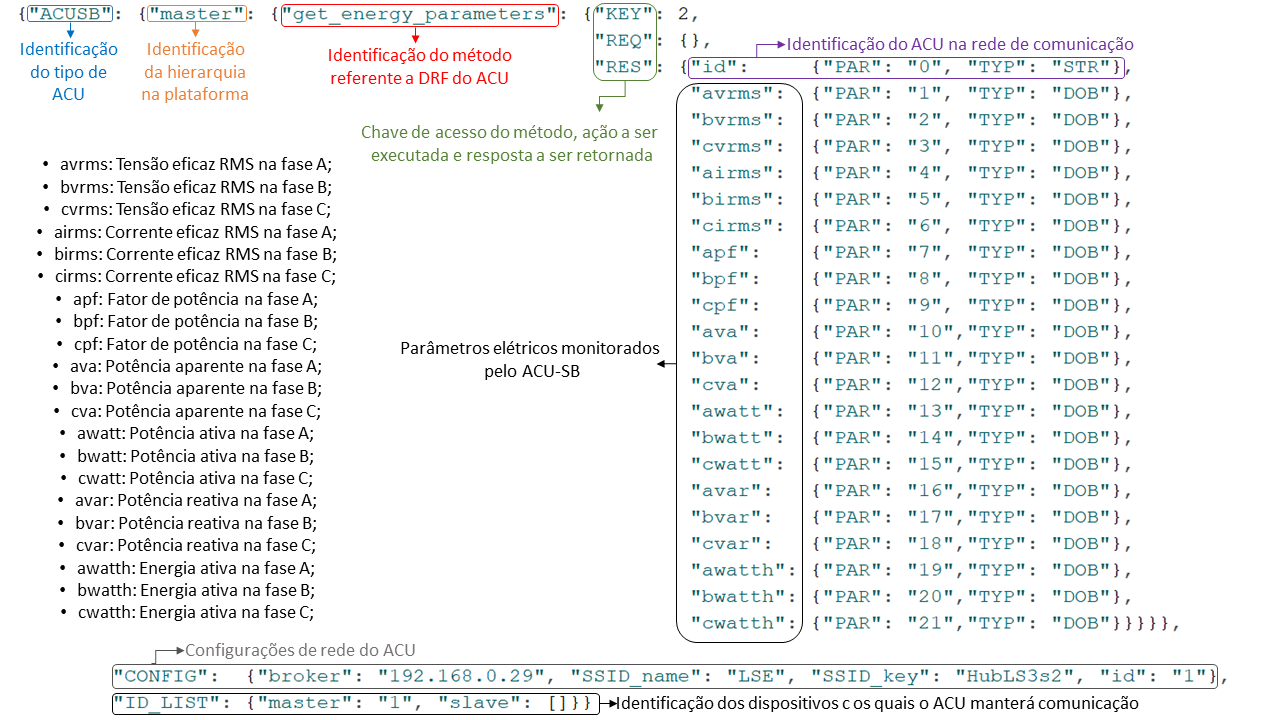
\includegraphics[width=0.95\linewidth]{img/jsonSB.png}
    \hspace{1cm}
    %\vspace{1cm}
	\legend{\small{Fonte: Autoria própria}}
\end{figure}
\end{frame}

\begin{frame}{Materiais e Métodos de Implementação}{A prototipagem dos ACUs}
\vspace{-0.64cm}
\begin{figure}[htp]
	\centering
	\caption{ \centering\small{{\textit{Layouts} e protótipos dos ACUs}}}
	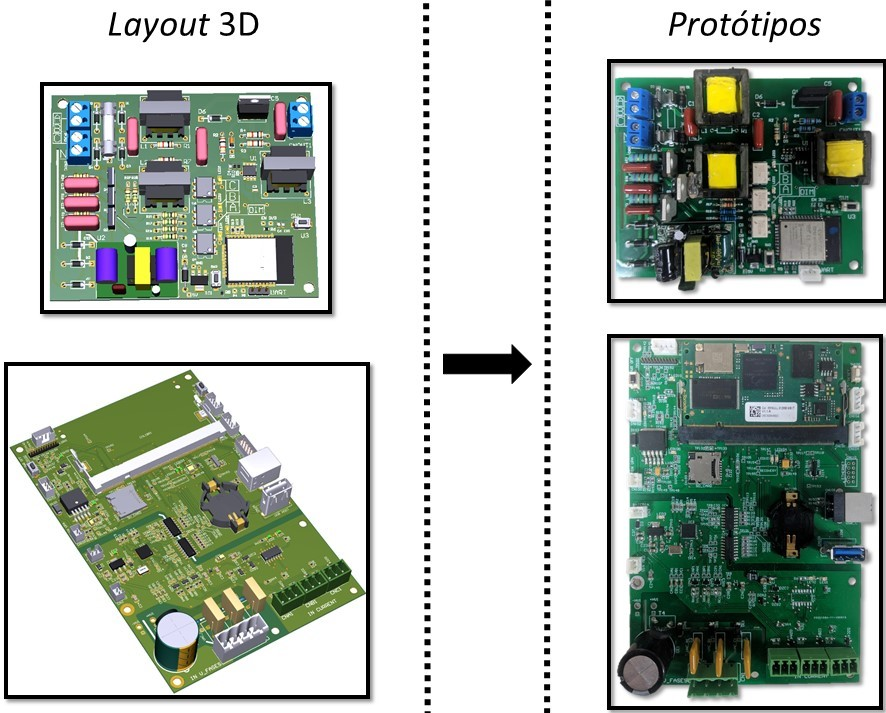
\includegraphics[width=0.68\linewidth]{img/prots.jpg}
    \hspace{5cm}
    \vspace{5cm}
	\legend{\small{Fonte: Autoria própria}}
\end{figure}
\end{frame}

\begin{frame}{Materiais e Métodos de Implementação}{A metodologia para execução do \textit{retrofit}}
\vspace{-0.64cm}
\begin{figure}[htp]
	\centering
	\caption{ \centering\small{{O \textit{retrofit} do ACU-LUM}}}
	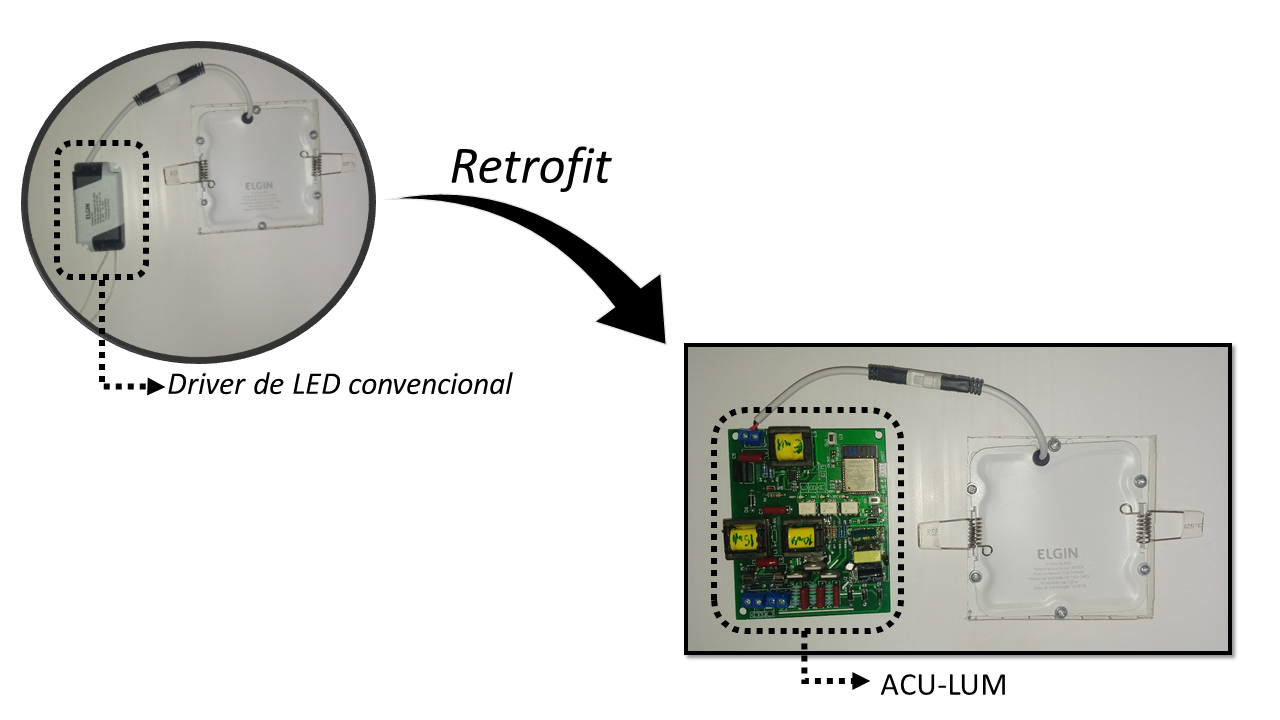
\includegraphics[width=0.98\linewidth]{img/retro_lum.png}
    \hspace{5cm}
    \vspace{1cm}
	\legend{\small{Fonte: Autoria própria}}
\end{figure}
\end{frame}

\begin{frame}{Materiais e Métodos de Implementação}{A metodologia para execução do \textit{retrofit}}
\vspace{-0.64cm}
\begin{figure}[htp]
	\centering
	\caption{ \centering\small{{O \textit{retrofit} do ACU-SB}}}
	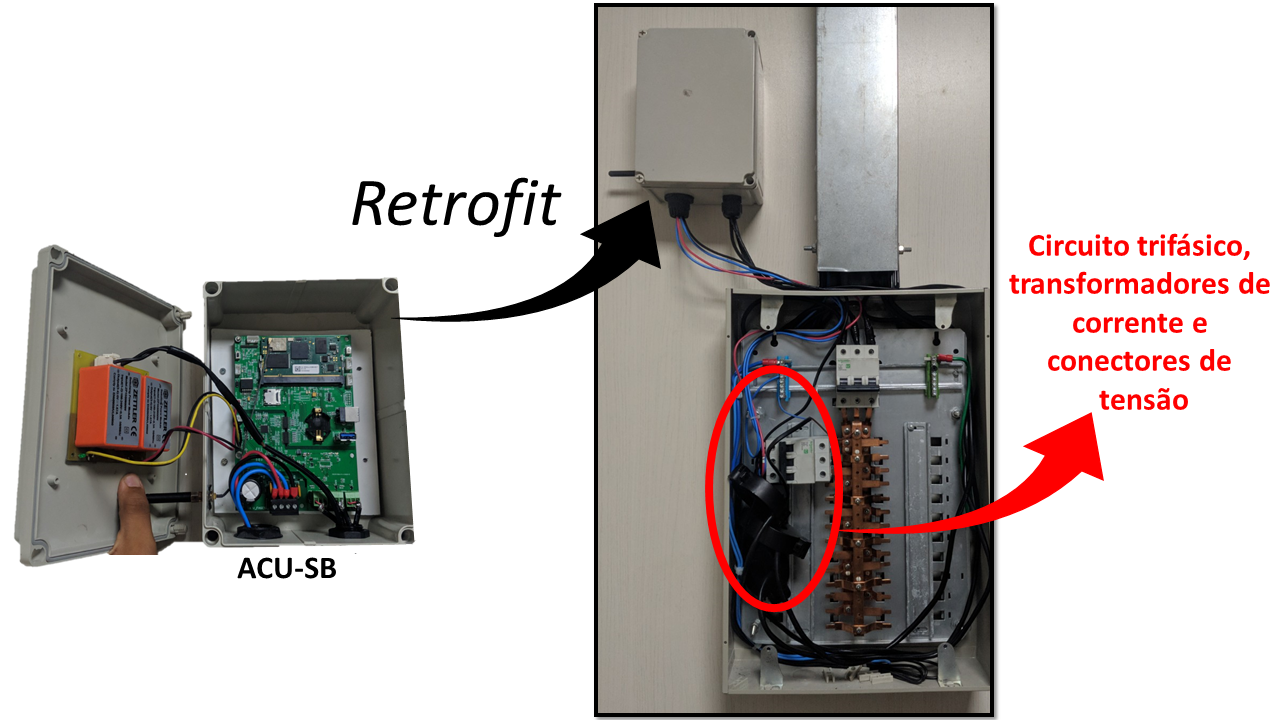
\includegraphics[width=0.95\linewidth]{img/retro_sb.png}
    \hspace{5cm}
    \vspace{1cm}
	\legend{\small{Fonte: Autoria própria}}
\end{figure}
\end{frame}
